\subsection{Reductions}

\begin{wrapfigure}{R}{0.6\textwidth}
\vspace{-0.5cm}
\begin{center}
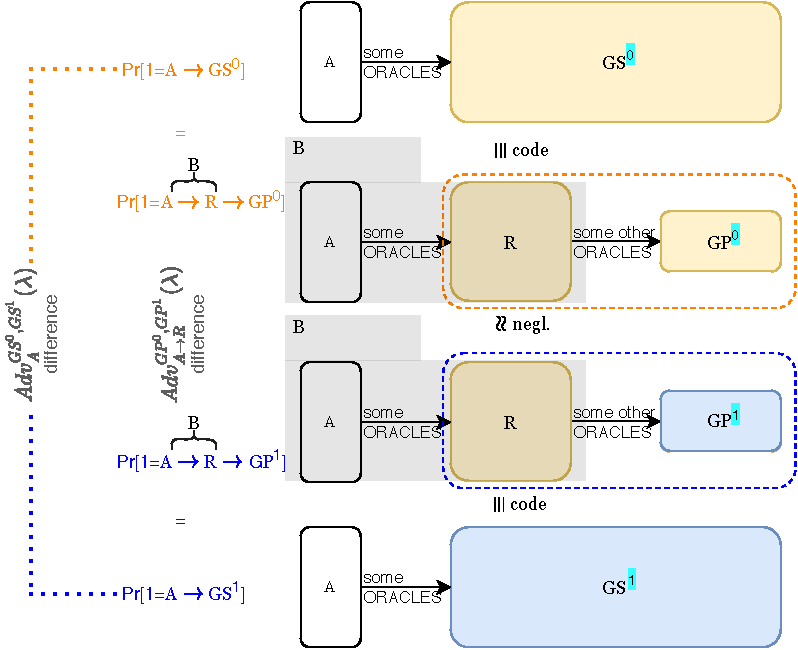
\includegraphics[width=0.6\textwidth]{figs/reduction}
\caption{\label{fig:reduction-example}New adversary $\bdv=\adv\circ\M{R}$}
\end{center}
\vspace{-0.5cm}
\end{wrapfigure}

In cryptography, we are often interested in proving the security of cryptographic systems or protocols. However, cryptography doesn't yet have methods of proving things secure from first principles (cf. the \textbf{P} vs. \textbf{NP} discussion in Section~\ref{ssec:assumptions}). Therefore, we are left with proving the security of systems \emph{assuming} that some (hopefully) well-understood and (typically) widely-used primitives are secure. Proofs of this type are done using reductions, which we explain in this section.

First, let's go over the general idea of a reduction proof.
Let's say that we want to prove the security of some system $S$, under the assumption that primitive $P$ is secure. In a reduction proof, we do this via a \emph{proof by contradiction}\footnote{Those familiar with formal logic will recognize this as modus ponens, i.e., $A\Rightarrow B$ is equivalent to $\neg B\Rightarrow \neg A$.} (which can take some time to get used to): we assume that $S$ is \emph{insecure} and prove that $P$ is then also insecure. If we can carry out such a proof, we can then argue that $S$ is secure. After all, if $S$ were insecure, then our proof would say that $P$ is also insecure, which is this in contradiction to our assumption that $P$ is \emph{secure}.

So, how do we prove that $S$ being insecure implies $P$ being insecure? Here it is important to realize what it means for $S$ to be insecure. It means that there is some (efficient) adversary $\adv$ that can break the security of $S$. Similarly, to prove that $P$ is insecure, we have to provide a new efficient adversary $\bdv$ that can break it. Due to our assumption of $\adv$ breaking $S$, we are allowed to use $\adv$ in the code of $\bdv$. As we don't know the \emph{code} of $\adv$, our construction of $\bdv$ needs to use $\adv$ in a black-box way. In particular, we can't make any assumptions about the precise functioning of $\adv$, except for knowing that $\adv$ breaks $S$.

Thus, we construct adversary $\bdv$ as a \emph{composition} of $\adv$ and a \emph{package} $\M{R}$, the latter of which we call reduction. A package is a generalization of the notion of a \emph{game} which we introduced in Section~\ref{ssec:security-games}. Namely, a package $\M{R}$ \emph{provides} oracles, denoted $[\rightarrow\M{R}]$, and also \emph{calls} oracles, denoted $[\rightarrow\M{R}]$. Now, in fact, an adversary can be seen as a package, too---it doesn't provide any oracles, it just calls some. So, e.g., to practice our language, we can say that $\adv$ and $\M{R}$ have \emph{matching} oracles and dependencies, namely $[\adv\rightarrow]=[\rightarrow\rdv]$, i.e., the oracles that $\adv$ calls are the oracles that $\M{R}$ provides. We use the $\rightarrow$ notation to write composition, namely, we define the adversary $\bdv$ as
\[\bdv:=\adv\rightarrow\M{R}.\]

We describe our reductions explicitly by giving the code of the oracles of the reduction. Namely, we consider the usual case that the security of $P$ is defined as the indistinguishability between a real game $\M{GP}^0$
and an ideal game $\M{GP}^1$. Let us further consider that the security of $S$ is defined as the indistinguishability between
a real game $\M{GS}^0$ and an ideal game $\M{GS}^1$. Then a reduction $\M{R}$ from the security of $S$ to the security of $P$
is an (efficient!) package $\M{R}$, written in pseudo-code. And we need that if $\adv$ is successful in distinguishing $\M{GP}^0$ and 
$\M{GP}^1$, then $\bdv:=\adv\rightarrow\M{R}$ is successful in distinguishing $\M{GS}^0$ from $\M{GS}^1$. The easiest case is,
if for all adversaries $\adv$, it holds that
\begin{equation}\label{lalaland1}
\mathsf{Adv}^{\M{GS}^0,\M{GS}^1}_\adv(\lambda)=\mathsf{Adv}^{\M{GP}^0,\M{GP}^1}_{\adv\rightarrow\M{R}}(\lambda).
\end{equation}
With Equation~\ref{lalaland} at hand, we can prove\footnote{See Lecture Notes 3 and Lecture Video 4, minutes 16:30 and 27:56, for a concrete such argument: The main reason that code equivalence implies that two games behave exactly the same and thus, and adversary has exactly the same probability against the two games. We use this argument a lot in this course.}  that for all adversaries $\adv$, it holds that 
and thus, if there is an efficient adversary $\adv$ which has non-negligible advantage against the pair $(\M{GS}^0,\M{GS}^1)$,
then there is also an efficient adversary $\adv\rightarrow\M{R}$ against the pair $(\M{GP}^0,\M{GP}^1)$ which has the same
advantage. However, we assume that there is no efficient $\bdv$ with non-negligible advantage $\mathsf{Adv}^{\M{GP}^0,\M{GP}^1}_{\bdv}$, thus taking $\bdv=\adv\rightarrow\M{R}$ leads to a contradiction. In conclusion, there cannot be an efficient $\adv$ such that $\mathsf{Adv}^{\M{GS}^0,\M{GS}^1}_\adv$ is non-negligible. The \emph{core argument}, here, is that (1) $\adv\rightarrow\M{R}$ is efficient (i.e., PPT) whenever $\adv$ is efficient, and (2) Equation~\ref{lalaland1}.

How can we prove that Equation~\ref{lalaland1} holds? We can show this by establishing that
\begin{align}
\notag          &\M{GS}^0\stackrel{\text{code}}{\equiv}\M{R}\rightarrow\M{GP}^0\text{ and }\\
\label{lalaland}&\M{GS}^1\stackrel{\text{code}}{\equiv}\M{R}\rightarrow\M{GP}^1,
\end{align}
that is, that $\M{GS}^0$ has the same input-output behaviour as $\M{R}\rightarrow\M{GP}^0$
and that $\M{GS}^1$ has the same input-output behaviour as $\M{R}\rightarrow\M{GP}^1$.
Because if this holds, then we can replace $\M{GS}^0$ by $\M{R}\rightarrow\M{GP}^0$
and $\M{GS}^1$ by $\M{R}\rightarrow\M{GP}^1$ and can prove Equation~\ref{lalaland1} as follows:
\begin{align*}
&\mathsf{Adv}^{\M{GS}^0,\M{GS}^1}_\adv(\lambda)\\
=&\abs{\prob{1=\adv\rightarrow\M{GS}^0}-\prob{1=\adv\rightarrow\M{GS}^1}}\\
=&\abs{\prob{1=\adv\rightarrow(\M{R}\rightarrow\M{GP}^0)}-\prob{1=\adv\rightarrow(\M{R}\rightarrow\M{GP}^1)}}\\
=&\abs{\prob{1=(\adv\rightarrow\M{R})\rightarrow\M{GP}^0}-\prob{1=(\adv\rightarrow\M{R})\rightarrow\M{GP}^1}}\\
=&\mathsf{Adv}^{\M{GP}^0,\M{GP}^1}_{\adv\rightarrow\M{R}}(\lambda)
\end{align*}
(Note that we usually don't write the brackets, we just include them here for emphasis.)

We now want to define the notion of a reduction formally. To do this, let us first include a formal definition of 
a \emph{package}.
\begin{definition}[Package]
A package $\M{R}$ consists of a set of oracles, denoted $[\rightarrow \M{R}]$,
which are defined by pseudo-code that operates on shared \emph{state variables} and makes calls to oracles in $[\M{R}\rightarrow]$,
which are called the \emph{dependencies} of $\M{R}$. Oracles in $[\rightarrow \M{R}]$
can only call oracles in $[\M{R}\rightarrow]$, they cannot call oracles in $[\rightarrow \M{R}]$.
(This is important for interpretation of code particularly if an oracle name $\O{O}$ is contained 
in $[\M{R}\rightarrow]$ and $[\rightarrow \M{R}]$.)
\end{definition}
\begin{definition}[Sequential Package Composition $\&$ Inlining]
If two packages $\M{R}$ and $\M{G}$ have \emph{matching interfaces}, i.e.,
$[\M{R}\rightarrow]\subseteq[\rightarrow\M{G}]$, then we can write
$\M{R}\rightarrow\M{G}$ for their composition which is defined by
inlining the code of the oracles of $\M{G}$ into the oracle of $\M{R}$,
i.e., if oracle $\O{O}\in[\rightarrow\M{G}]$ is defined as $\textit{code}(x);\pcreturn a$
and the pseudocode of oracle $\O{O}'\in[\rightarrow\M{R}]$ contains the line
$b\gets \O{x}$, then this line is replaced by $b\gets\textit{code}(x)$. Note that
when inlining, state variables might need to be renamed in order to avoid collisions.
\end{definition}

While Equation~\ref{lalaland1} was crucial in our argument, let us reflect on whether we need the actual Equation~\ref{lalaland1} or whether there are variants of it that would suffices. Actually, we only need an argument which justifies that if $\mathsf{Adv}^{\M{GS}^0,\M{GS}^1}_\adv$ is non-negligible, then $\mathsf{Adv}^{\M{GP}^0,\M{GP}^1}_{\adv\rightarrow\M{R}}$ is non-negligible. Any of the following inequalities would establish this desired result as well:
\begin{align*}
\mathsf{Adv}^{\M{GS}^0,\M{GS}^1}_\adv(\lambda)&\leq\mathsf{Adv}^{\M{GP}^0,\M{GP}^1}_{\adv\rightarrow\M{R}}(\lambda)\\
\mathsf{Adv}^{\M{GS}^0,\M{GS}^1}_\adv(\lambda)&\leq 2\cdot\mathsf{Adv}^{\M{GP}^0,\M{GP}^1}_{\adv\rightarrow\M{R}}(\lambda)\\
\mathsf{Adv}^{\M{GS}^0,\M{GS}^1}_\adv(\lambda)&\leq \O{poly}(\lambda)\cdot\mathsf{Adv}^{\M{GP}^0,\M{GP}^1}_{\adv\rightarrow\M{R}}(\lambda)\\
\mathsf{Adv}^{\M{GS}^0,\M{GS}^1}_\adv(\lambda)&\leq \O{poly}(\lambda)\cdot\sqrt{\mathsf{Adv}^{\M{GP}^0,\M{GP}^1}_{\adv\rightarrow\M{R}}(\lambda)}\\
\mathsf{Adv}^{\M{GS}^0,\M{GS}^1}_\adv(\lambda)&\leq \O{poly}(\lambda)\cdot\sqrt[5]{\mathsf{Adv}^{\M{GP}^0,\M{GP}^1}_{\adv\rightarrow\M{R}}(\lambda)}
\end{align*}
The reason that all of these inequalities work is that by multiplying (or dividing) by constants, polynomials and squaring (or taking square roots), a negligible function cannot become non-negligible (or vice versa). We are almost ready to state the notion of a reduction, but actually, we still need to make this statement a bit more general. The reason is that often, we have more than one algorithm $\M{R}$, and, e.g., might have inequalities such as 
\begin{equation}\label{lalaland12}
\mathsf{Adv}^{\M{GS}^0,\M{GS}^1}_\adv(\lambda)=\mathsf{Adv}^{\M{GP}^0,\M{GP}^1}_{\adv\rightarrow\M{R}_1}(\lambda)+\mathsf{Adv}^{\M{GP}^0,\M{GP}^1}_{\adv\rightarrow\M{R}_2}(\lambda),
\end{equation}
for two different, efficient $\M{R}_1$ to $\M{R}_1$. This equation still suffices, since the sum of two negligible functions is negligible again, and if $\mathsf{Adv}^{\M{GS}^0,\M{GS}^1}_\adv$ was non-negligible, then $\mathsf{Adv}^{\M{GP}^0,\M{GP}^1}_{\adv\rightarrow\M{R}_1}$ or 
$\mathsf{Adv}^{\M{GP}^0,\M{GP}^1}_{\adv\rightarrow\M{R}_2}$ would need to be non-negligible. As you can imagine, we can also combine this flexibility: Have \emph{several} efficient $\M{R}_i$ and some complex equation. To cross-refer to the lectures, let me mention here an inequality which we use in Lecture Notes 4:
\begin{align}
   \notag&\mathsf{Adv}^{\M{Gunf\text{-}cma}_{\m_f}^0,\M{Gunf\text{-}cma}_{\m_f}^1}_{\m_f,\adv}(\lambda)\\
   \notag\leq&\mathsf{Adv}^{\M{Gprf}^0,\M{Gprf}^1}_{f,\adv\rightarrow\M{R}_1}(\lambda)\\
	       &\label{lalaland123}+\mathsf{Adv}^{\M{Gprf}^0,\M{Gprf}^1}_{f,\adv\rightarrow\M{R}_2}(\lambda)+\frac{\O{poly}_{\adv}(\lambda)}{2^\lambda},
\end{align}
Here, we add two advantages and some negligible term $\frac{\O{poly}_{\adv}(\lambda)}{2^\lambda}$, where $\O{poly}_{\adv}$ is
some polynomial which depends on the adversary (in this case an upper bound on the number of queries that $\adv$ makes).
Thus, also Inequality~\ref{lalaland123} suffices to establish that if there is no efficient adversary such that 
\[\mathsf{Adv}^{\M{Gprf}_f^0,\M{Gprf}_f^1}_{f,\bdv}\] is non-negligible, then there is also no efficient adversary such
that \[\mathsf{Adv}^{\M{Gunf\text{-}cma}_{\m_f}^0,\M{Gunf\text{-}cma}_{\m_f}^1}_{\m_f,\adv}\] is non-negligible.

\begin{quote}
How do we know which combination is the right one in which situation?
\end{quote}

We don't really know this. Moreover, there are
often more than one right way to do this. In essence, any approach that works is good, and we will see many such
examples of proofs in this book,
 so they will hopefully become familiar over time.

Let us now state the notion of a reduction:
\begin{definition}[Reduction]
We call a package $\M{R}$ a reduction from the indistinguishability of $\M{GS}^0$ and  $\M{GS}^1$ to the indistinguishability of 
$\M{PS}^0$ and  $\M{PS}^1$, if
\begin{itemize}
\item $\M{R}$ is efficient, i.e., probabilistic polynomial-time (PPT), and
\item for any efficient adversary $\adv$, it holds that if $\mathsf{Adv}^{\M{GS}^0,\M{GS}^1}_\adv$ is non-negligible, then
      $\mathsf{Adv}^{\M{GP}^0,\M{GP}^1}_{\adv\rightarrow\M{R}}$ is non-negligible.
\end{itemize}
Additionally, we call two packages $\M{R}_1$ and $\M{R}_2$ reductions from the indistinguishability of $\M{GS}^0$ and  $\M{GS}^1$ to the indistinguishability of 
$\M{PS}^0$ and  $\M{PS}^1$, if
\begin{itemize}
\item $\M{R}_1$ and $\M{R}_2$ are efficient, i.e., probabilistic polynomial-time (PPT), and
\item for any efficient adversary $\adv$, it holds that if $\mathsf{Adv}^{\M{GS}^0,\M{GS}^1}_\adv$ is non-negligible, then
      $\mathsf{Adv}^{\M{GP}^0,\M{GP}^1}_{\adv\rightarrow\M{R}_1}$ or $\mathsf{Adv}^{\M{GP}^0,\M{GP}^1}_{\adv\rightarrow\M{R}_2}$ is non-negligible.
\end{itemize}
In this case, we refer to $\M{R}_1$ and $\M{R}_2$ as a reductions, even though one of them alone does not match the first
part of the definition.
\end{definition}
Potentially, we could have also more than two reductions $\M{R}_i$, but we are not aware of any such example,
so we do not generalize the definition.


\iffalse
So, how do we prove that $S$ being insecure implies $P$ being insecure? Here it is important to realize what it means for $S$ to be insecure. It means that there is some adversary $\adv$ that can break the security of $S$. Similarly, to prove that $P$ is insecure, we have to provide an adversary $R$ that can break it. However, due to our assumption, we are allowed to use $\adv$ in the code of $R$. Note that we don't know the \emph{code} of $\adv$, so $R$ can only use $\adv$ in a black-box way, and we can't make any assumptions about the precise functioning of $\adv$.

Reduction proofs can be carried out explicitly, by defining $R$ in pseudocode. However, a major benefit of the framework we're using is to simplify proofs of this type. Often, we can do a reduction proof just using package composition diagrams for the two systems in question. This is because the reductions we want to construct are often simply some part of the package composition we are working with. The next section does reduction proofs in detail, so reading those might be the best way of getting to grips with this idea. Here, we will only discuss the idea in general, algebraic terms. Figure~\ref{fig:reduction-example} presents the situation graphically, so you might like to look at it while reading the following.

\begin{wrapfigure}{R}{0.6\textwidth}
\vspace{-0.5cm}
\begin{center}
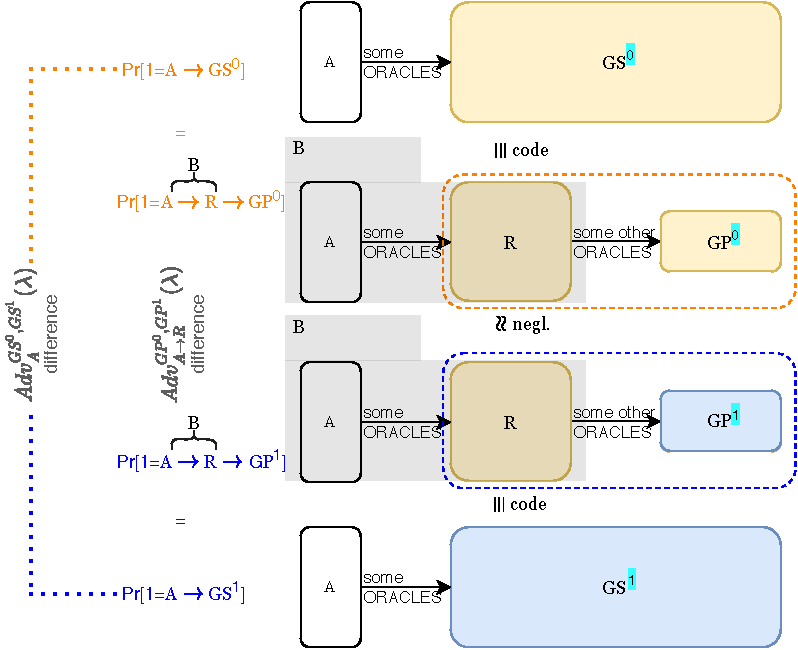
\includegraphics[width=0.6\textwidth]{figs/reduction}
\caption{\label{fig:reduction-example}Reduction $\rdv=\adv\circ\M{N}$}
\end{center}
\vspace{-0.5cm}
\end{wrapfigure}

Let us say we are trying to prove that some system $S$ is secure assuming that primitive $P$ is secure. Let us further posit that security of  $S$ is defined by indistinguishability of the real and ideal games $\M{S}^0$ and $\M{S}^1$, depicted in orange and blue, respectively. Similarly, consider that the security of $P$ is defined by the indistinguishability of the real game $\M{P}^0$ and the ideal game $\M{P}^1$. Now, we set out to prove that $P$ is insecure assuming that $S$ is. The assumption gives us an adversary that can break the security of $S$. This means, specifically, that the composition $\adv\circ\M{S}^0$ returns $1$ with much higher (or much lower) probability than the composition
$\adv\circ\M{S}^1$ so that the difference between these two probabilities is some high enough value $\epsilon$. Now, let us say that we can re-write $\M{S}^0$ as $\M{N}\circ\M{P}^0$ for some package $\M{N}$ and let us consider the situation that $\M{S}^1=\M{N}\circ\M{P}^1$ for the same package $\M{N}$. Now, we can rewrite the $\M{S}^0$ and $\M{S}^1$ into $\M{N}\circ\M{P}^0$ and $\M{N}\circ\M{P}^1$ (illustrated by orange and blue dashed lines, respectively). As the systems still behave the same, the probabilities remain unchanged and $\epsilon$ is now also the difference between $\adv \circ \M{N} \circ \M{P}^0$ returning $1$ and $\adv \circ \M{N} \circ \M{P}^1$ returning $1$.

Now, we can construct our reduction $R$: it is simply $\adv \circ \M{N}$. If the composition $\adv \circ (\M{N} \circ \M{P}^b)$ returns $1$, so must the composition $(\adv \circ \M{N}) \circ \M{P}^b = R \circ \M{P}^b$. Thus, in conclusion, we can argue that the security of $S$ (i.e., an adversary's distinguishing advantage between $\M{S}^0$ and $\M{S}^1$) is equal to the security of $P$ (i.e., the distinguishing advantage of a different adversary between $\M{P}^0$ and $\M{P}^1$). 

This is the general form that reduction proofs in this course follow. The problem often is not so simple, i.e., sometimes, we need to consider two slightly different packages $\M{N}$ and $\M{N'}$ which actually behave in the same way (or almost the same way) but have slightly different code. In this case, the same type of argument still goes through as long as we can show that $\M{N}$ and $\M{N'}$ are \emph{code-equivalent}. 
\fi

We already mentioned the technique of proving \emph{code-equivalence} several time. We turn to code-equivalence in the next section.